\section{Metrics}

The following section illustrates some facts about the application in terms of metrics. 

\subsection{Github metrics}

The image below is a screenshot from the github repository in which the application has been created.
There were 472 commits done, scattered across 50 branches.

\begin{center}
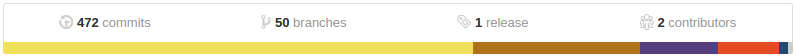
\includegraphics[scale=0.5]{./img/github_stats.png}
\end{center}

During the development of the application a set of conventions were agreed upon, which included keeping a clean
branching tree within the repository. The image below illustrates the last few merges with the master branch.

\begin{center}
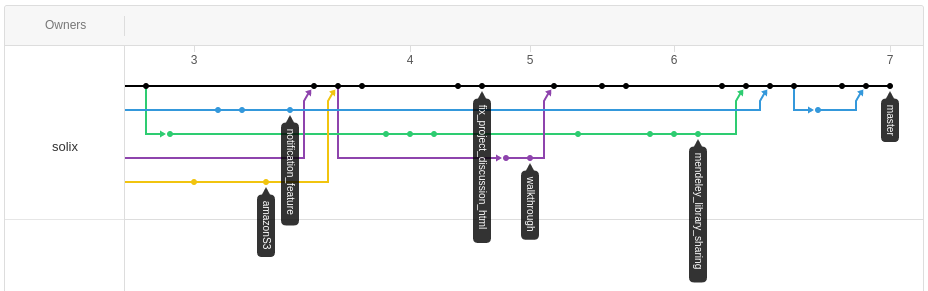
\includegraphics[scale=0.5]{./img/github_tree.png}
\end{center}

\subsection{Application metrics}

The following metrics illustrate the size and quality of the application.

\begin{itemize}
	\item Total lines of code: \textbf{5341} (including statically imported plugins)
	\item Total code coverage: \textbf{69\%} (excluding statically imported plugins and framework code)
\end{itemize}